\documentclass{article}
\usepackage[UTF8]{ctex}
\usepackage{geometry}
\usepackage{multirow}
\usepackage{natbib}
\geometry{left=3.18cm,right=3.18cm,top=2.54cm,bottom=2.54cm}
\usepackage{graphicx}
\pagestyle{plain}	
\usepackage{setspace}
\usepackage{enumerate}
\usepackage{caption2}
\usepackage{datetime} %日期
\renewcommand{\today}{\number\year 年 \number\month 月 \number\day 日}
\renewcommand{\captionlabelfont}{\small}
\renewcommand{\captionfont}{\small}
\begin{document}

\begin{figure}
    \centering
    
\includegraphics[width=8cm]{upc.png}

    \label{figupc}
\end{figure}

	\begin{center}
		\quad \\
		\quad \\
		\heiti \fontsize{45}{17} \quad \quad \quad 
		\vskip 1.5cm
		\heiti \zihao{2} 《计算科学导论》个人职业规划
	\end{center}
	\vskip 2.0cm
		
	\begin{quotation}
% 	\begin{center}
		\doublespacing
		
        \zihao{4}\par\setlength\parindent{7em}
		\quad 

		学生姓名:\underline{\qquad  高启东 \qquad \qquad}

		学\hspace{0.8cm} 号:\underline{\qquad 1907010121\qquad}
		
		专业班级:\underline{\qquad 计科1901 \qquad  }
		
        学\hspace{0.8cm} 院:\underline{计算机科学与技术学院}
% 	\end{center}
		\vskip 1.5cm
		\centering
		\begin{table}[h]
            \centering 
            \zihao{4}
            \begin{tabular}{|c|c|c|c|c|c|c|c|c|}
            % 这里的rl 与表格对应可以看到,姓名是r,右对齐的;学号是l,左对齐的;若想居中,使用c关键字。
                \hline
                \multicolumn{5}{|c|}{分项评价} &\multicolumn{2}{c|}{整体评价}  & 总    分 & 评 阅 教 师\\
                \hline
                自我 & 环境 & 职业 & 实施 & 评估与 & 完整性 & 可行性 &\multirow{2}*{} &\multirow{2}*{}\\
                分析& 分析& 定位 & 方案 & 调整 & 20\% & 20\% & ~&~ \\\            
                10\% & 10\% & 15\% & 15\% & 10\% & &  &~ &~\\
                \cline{1-7} 
                & & & & & & & ~&~ \\
                & & & & & & & ~&~ \\
                \hline      
            \end{tabular}
        \end{table}
		\vskip 2cm
		\today
	\end{quotation}

\thispagestyle{empty}
\newpage
\setcounter{page}{1}
% 在这之前是封面,在这之后是正文
\section{自我分析}
	%自我分析即对自己进行全方位、多角度的分析,目的是认识自己、了解自己。只有认识了自己,才能对自己的职业做出正确的选择,才能选定适合自己发展的职业生涯路线,才能对自己的职业生涯目标做出最佳抉择。\par
	%自我分析包括:\par
\subsection{自然条件}
性别:男\par
年龄:18\par
身体状况:良好\par
健康状况:健康\par
居住城市:家乡:甘肃省景泰县\par
          学校:青岛市 中国石油大学(华东)\par 
%性别、年龄、身体条件、健康状况、居住城市等。\par
\subsection{性格分析}
\par
我的性格有点偏内向,但挺喜欢和别人交流。在生活中,我也喜欢研究一些感兴趣的、新奇的事物或技术,常常在研究某个东西时,熬夜到很晚。我觉得这是一个不错的品质,应该值得发扬。但我在耐力、和坚持上做的并不好。如,在某件事上,常常不能坚持很长一段时间,或者在遇到某些难题或瓶颈时,会常常不能狠下心去攻克,而是会轻易放弃,我觉得这是我性格上最大的缺陷之一。以后可能会因为这个错失许多发展的机会,所以应该积极改变。\par
再者,我经常会遇事不决,也有所谓的“选择恐惧症”,例如,我在遇到许多事情时,常常会想的太多,犹豫不定,导致我错过了许多机会,因此为了以后能拥有更多的机会,这也是需要积极改变的性格之一。
\par
\subsection{教育与学习经历}
\par
9岁以前,住在大山里,在村里的小学读书;\par
9岁时,家庭搬迁,由于本村规模小,没有学校,去邻村读的小学后半段;\par
初中时,我去了镇上的学校,成绩也能在班级中名例前茅;\par
中考后,去了高中比较好的班级,成绩也可以;\par
高考后,考入中国石油大学(华东)。\par
\subsection{工作与社会阅历}
\par
说起工作,其实我并没有参加过什么正式的工作,也仅仅是在家帮父母干干农活,而且,我也并是很不喜欢走出家门,接触到的人也不是很多,因此也基本没什么社会履历。
\subsection{知识、技能与经验}
\par
目前掌握了C++的基础语法,会C++的基本操作,也了解了LaTex的相关基础知识,并且可以借助网络、书籍等达到自己的编写目的。现在也开始提前了解Web前端开发以及Python的内容。
\subsection{兴趣爱好与特长}
\par
我比较喜欢与计算机、网络有关的技术,并且也加入了学校ACM后备营,积极学习有关算法,并且积极了解相关技术的基础知识。\par
说起特长,其实我觉得我并没有什么特长,可能比较好的一方面就是愿意投入大量时间和精力去做自己喜欢的事情,并会通过书籍、网络、IT网站、社区等途径钻研它们。
\section{环境分析}
%环境分析主要是评估周边各种环境因素对自己职业生涯发展的影响。每一个人都处在一定的环境之中,职业发展必然要受到所处环境的影响,只有充分了解和把握所处环境的现状、特点、发展变化趋势,才能做到在复杂的环境中避害趋利,使你的职业生涯规划具有实际意义。\par
环境分析包括:\par
\subsection{社会环境分析}
\subsubsection{政治形势}
中国面临的机遇和挑战在世界格局新旧交替之际,中国所面临的外部形势是机遇和挑战并存。从机遇方面看,两极格局的瓦解,世界局势的缓和,改善了中国的国际环境;在多极格局中,中国对国际战略平衡的影响,已比过去增强,中国的国际地位和作用也得到提高。特别是在亚太地区建立新的政治、经济合作体系,没有中国的参与是不可能实现的。从挑战方面看,首先是随着世界经济区域集团化,保护主义盛行,中国的对外经济面临着激烈的竞争。其次,在经济全球一体化的趋势下,世界各国尤其是发达资本主义国家经济形势的变化,也给中国的经济发展带来一定程度的制约。再次,少数发达国家推行一种新的强权政治,施加种种压力,企图迫使中国放弃社会主义。在这种情况下,中国只有坚持独立自主、建设有中国特色的社会主义的道路,才能利用有利因素,抵制外来的不利影响,抓住机遇,迎接挑战,尽快建成社会主义现代化国家。\par
\subsubsection{经济形势}
中国所处国际经济环境呈现了新趋势。经济全球化的发展趋势对世界产生了巨大冲击,也必定会对21 世纪的国际形势产生重大影响。一方面全球化促进了世界范围的经济增长与繁荣,打破了旧有的国际政治地图。由于对外开放,中国事实上已经加入了世界经济体系,中国大陆本身日益成为全球的一个最大市场之一。应当看到,科学技术的迅猛发展和经济全球化,为中国实现社会主义现代化提供了机遇。首先,它使它们更全面、更广阔地去了解世界上各种经济体制的优点和缺点,市场经各种模式的利与弊,从而为中国经济体制改革提供更多的借鉴和选择。\par
\subsubsection{就业形势}
从总量上看,劳动力供给增速趋缓,总量逐步减少,总量压力相对缓解,但仍然高位持压。2012年开始,我国劳动年龄人口数量持续下降,与以往高速增长的发展趋势明显不同,就业总量的压力从增量向存量转变。但未来相当长一段时间,我国的就业总量仍将处于一种持续中高压状态。据测算,到2030年之前我国16~59岁的劳动年龄人口仍将一直保持在8亿以上。\par
从结构上看,就业结构性矛盾不断上升。与改革开放初期和国有企业改革攻坚阶段出现的就业结构性矛盾不同,当前就业结构性矛盾是在经济社会发展持续转型到一定阶段时形成的,劳动力的需求和供给结构都存在显著的转型特征。\par
就业结构性矛盾是经济社会发展不协调、不平衡的结构性问题在就业领域的集中反映。其既有产业结构调整和技术进步的因素,也有区域经济格局变化的影响,如城乡二元结构逐渐被打破,但体制分割没有完全消除;各地区发展迅速但仍然很不平衡;居民收入水平上升但仍然差距巨大;劳动者社会横向流动过于频繁,而纵向流动困难。但最根本的还是劳动力需求和供给的不匹配。\par
%政治形势、经济形势、就业形势等。\par
\subsection{家庭环境分析}
未婚,经济来源主要是父母。父母及家人对我的期望挺大的,他们希望我能努力学习知识,以后可以在一个好一点的环境工作,同时,他们也希望我将来能够运用自己所学的知识,充分发挥自己的能力,为祖国的高新技术发展和建设贡献自己的力量。
%婚姻状况、经济状况、家人期望、家族传统等。\par
\subsection{职业环境分析}
\begin{enumerate}
\item[1.] 行业现状及发展趋势:行业整体增速持续提升,预计全年软件业收入增速仍将维持在14\%以上。软件行业整体具有后周期性,因此预计随着国家经济的逐步复苏,软件行业整体的景气度将维持。在外部环境不确定性加大的情况下,国家不断推进大数据、互联网+、人工智能等新兴产业发展,自主可控将是未来发展的主要方向,国产软件在传统产业中的渗透率将会不断提升,传统产业转型升级的浪潮不可逆转,而软件和信息技术对传统产业转型升级的带动作用极为明显,因此预计未来的软件升级和应用需求将会保持较高景气度(如下图)。不仅如此,其也推动了很多领域的发展,如影视制作、教育方面、医疗技术、刑侦破案方面等。\citep{申子明2019计算机应用现状与计算机发展趋势}
\begin{figure}[!h]
\centering
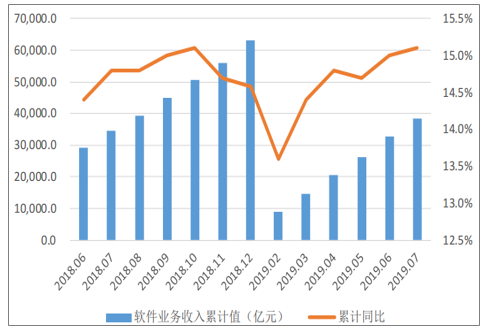
\includegraphics[scale=0.4]{ruanjian}
\caption{2018年6月-2019年7月我国软件业务收入累计值和同比增速}
\end{figure}
\item[2.] 职业的工作内容、工作要求、发展前景:\par
随着计算机行业岗位的细分,将该行业主要分为设计与开发、测试、UI、产品经理、运维和安全等岗位,每一个岗位都有其存在的不可替代性。\par
\begin{itemize}
\item  设计与开发:主要指从事代码撰写类的岗位,如:架构师、web前端、web后端、算法工程师、数据库工程师、手机程序员等等。\par
架构师:架构师的职责是开展软件的整体架构设计,站在顶层的角度,对软件的开发、未来发展方向等具有决定性影响力。\par
\item web前端: Web前端开发技术包括三个要素:HTML、CSS和JavaScript,这些都是计算机语言,学习起来并不难。web 前端入门容易后面进一步提升比较难,需要有美工、工业设计等等学科的支撑。\par
\item web 后端:web后端工程师主要实现业务逻辑, 提供接口给前端使用,或者说是给前端提供数据。服务端工程师做数据处理并把数据提供给前端用于显示出来。前端与后端,类似于计算机显示器和计算机主机的关系,计算机真正的运算是在主机(后端)当中进行的,运算完毕后,把数据输出到显示器(前端)显示出来。\par
\item 算法工程师:算法工程师是完成特定问题求解的工程技术人员,例如深度学习算法、机器学习算法,数据挖掘技术,自然语言处理技术,分布式计算等等。\par
\item 数据库工程师:几乎所有的软件都需要有数据库的支撑,完成结构化数据和非结构化数据的存储、访问和修改等操作,这都需要有数据库工程师的支撑。\par
\item 手机端程序员:主要是完成 Android 系统,和苹果 iOS 系统软件的设计开发。在手机几乎普及化的今天,手机软件开发成了当前的热门。Android 手机开发主要用 java 语言,iOS 系统软件开发主要用苹果自有的swift 语言。\par
\item 测试工程师:软件写完后,总是会有很多漏洞或者 bug 存在,为了找出这些缺陷,需要软件测试人员采用各种方式对软件进行全方位测试,确保交出去的软件足够强壮,不会轻易遇到 bug 后崩溃导致计算机蓝屏。随着技术发展,现在软件公司主要采用一系列的自动化测试工具对软件缺陷进行测试。行业对于测试人员的要求也在逐年提高。\par
\item UI:主要负责软件的界面美化,随着行业发展,也需要美工人员需要一定的计算机编程能力,设计好界面持续模板后,由前端工程师调用即可。这个工作,最适合学美术的人员来完成。\par
\item 产品经理:产品经理的主要职责,就是把用户的需求转化成程序员们能听懂的语言,并讲给他们听。行业知识是产品经理最重要的能力,产品经理可以不会编程,但一定要能懂行业,或者是拥有能快速了解行业的能力。 \par
\item 运维:运行维护的检查。一个大的公司网站或者软件系统建立并运行起来后,有可能会遇到很多故障或者 bug,就需要由运维人员完成日常的运行维护工作,公司越大,运维工程师就越重要。\par
\item 网络安全:在信息化时代,最重要的就是个人信息安全。网络安全工程师就是负责完成网络的漏洞发现、修补、病毒木马查杀等工作,确保安全无虞。\par
\end{itemize}
\end{enumerate}
%行业现状及发展趋势;职业的工作内容、工作要求、发展前景等。\par
\subsection{地域与人际环境分析}
就目前来说,我比较喜欢杭州这个城市。杭州位于中国华东地区、东南沿海、浙江省北部,是环杭州湾大湾区核心城市。它位于亚热带季风区,属于亚热带季风气候,四季分明,雨量充沛,夏季炎热、湿润,冬季寒冷、干燥,春秋气候宜人。而且其风景秀丽,素有“人间天堂”的美誉。\par
提起杭州,必然能想到西湖,西湖是杭州的象征,比较集中地体现了杭州的文化特色,所以杭州城市文化特色又称为“西湖文化”,它主要表现在四个方面:\begin{itemize}
\item[(1)]历史悠久,底蕴深厚;
\item[(2)]开放兼容,形态丰富;
\item[(3)]雅俗相融,自然和谐;
\item[(4)]优美秀丽,现代风范。
\end{itemize}
\par
新世纪以来,随着阿里巴巴等高科技企业的带动,互联网经济成为杭州新的经济增长点。所以杭州的IT行业的发展前景是比较乐观的。\par
目前暂无人脉与人际关系。
%工作城市的气候水土、文化特点、发展前景;人脉与人际关系等。\par
%图片插入的样例:\par
%\begin{figure}[h!]
%\centering
%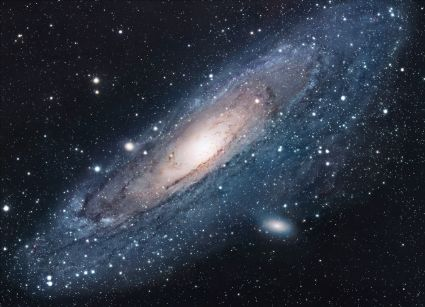
\includegraphics[scale=1.7]{universe}
%\caption{The Universe}
%\label{fig:universe}
%\end{figure}

\section{职业定位}
%在准确地对自己和环境做出了分析之后,确定适合自己行业和有实现可能的职业发展目标。职业定位时要注意与自己的自然条件、知识背景、技能特长、性格特点、兴趣爱好是否匹配,考虑与自己所处的环境是否相适应。职业定位决定了职业发展中的行为和结果,是制定职业生涯规划的关键,应当科学合理,具有可行性。\par
%职业定位包括:\par

\subsection{行业领域定位与理由}
\par
从事领域:人工智能领域。\par
理由:当今世界人工智能技术无论是在核心技术,还是典型应用上都已出现爆发式的进展。随着平台、算法、交互方式的不断更新和突破,人工智能技术的发展将主要以“AI+X”(为某一具体产业或行业)的形态得以呈现。所有这些智能系统的出现,将会改变某些职业模式。如今人工智能已经应用到各个方面:\par
\begin{itemize}
\item[1.]在我们生活方面,协助人类完成此前被认为必须由人完成的智能任务。
\item[2.]在生产方面,未来人工智能有望在传统农业转型中发挥重要作用。
\item[3.]在制造业中,人工智能将可以协助设计人员完成产品的设计,在理想情况下,可以很大程度上弥补中高端设计人员短缺的现状,从而大大提高制造业的产品设计能力。
\item[4.]在生活服务方面,人工智能同样有望在教育、医疗、金融、出行、物流等领域发挥巨大作用。
\item[5.]对金融而言,人工智能将能协助银行建立更全面的征信和审核制度,从全局角度监测金融系统状态,抑制各类金融欺诈行为,同时为贷款等金融业务提供科学依据,为维护机构与个人的金融安全提供保障。
\end{itemize}
\par
除了人工智能良好的发展前景,我本身也对其有很大的兴趣,所以我将来可能会从事与人工智能有关的职业。
\subsection{职业岗位起点定位与理由}
\par
起点:初级程序员\par
理由:先从最基础的岗位做起,逐渐提升自己能力,再向更高的层次发展。
\subsection{职业目标与可行性分析}
\par
%成果目标、经济目标、能力目标、职务目标等。\par 
\begin{enumerate}[1.]
	\item 短期目标:(大学4年)
\begin{itemize}
    \item 熟练掌握C/C++、python、Java等基础计算机编程语言;
    \item 能合理使用计算机语言完成自己的开发任务;
    \item 学习Web前端、后端的基础知识,并能做一些开发;
    \item 学习课外知识,了解各种计算机技术方面的知识,多方位,全方面地发展自身能力。
\end{itemize}
	\item 中长期目标:(5-10年)
\begin{itemize}
    \item 找到一个自己喜欢的工作;
    \item 对自己研究领域的内容有一个系统的、全面的认知,并能做一些复杂的开发;
    \item 能够积极发现市场需求,并能快速投入到相关的开发中。
\end{itemize}
%\end{enumerate}
%这里是简单列表的样例:(如果需要标号自定义或者自动标记数字序号,请自行搜索语法)
%\begin{itemize}
 %   \item 简单的列表结构 
  %  \item 如这里所示
   % \item 此处仅为样例
    %\item 按需修改和使用
%\end{itemize}


\section{实施方案}
%在明确了职业定位后,要制定实现职业生涯目标的行动方案,不付诸行动,职业目标只能是一种梦想。实施方案是实现职业目标的保证,尽量考虑周全、具有可操作性。\par
%实施方案可以从以下角度考虑:\par
\begin{enumerate}[1、]
	\item 在校期间,利用假期、周末及空闲时间更新知识,努力跟紧时代发展的潮流,积极主动参阅文献,合理利用书籍、IT网站来提高自己的综合能力。
	\item 积极改善自己的缺点,培养持之以恒和精神和坚韧不拔的意志,既要通过学习弥补知识上的空缺,也要通过大量实践弥补能力上的不足。
	\item 多于别人交流,通过借鉴别人的学习方法来完善自己的学习方法,多于技术大牛交流,逐渐完善自己的知识体系。
	\item 尽量做到家庭与事业兼顾,把握“在生活中工作”的基本原则,享受工作、享受生活。
	\item 积极参加体育运动,在运动中释压。
\end{enumerate}
\par  
%表格插入样例(三线表):\par
%单元格怎么写?参考第一页打分的表格

%\begin{table}[h]
%	\centering
%	\caption{这是科学系的花名册}
%	\begin{tabular}{rl}
		% 这里的rl 与表格对应可以看到,姓名是r,右对齐的;学号是l,左对齐的;若想居中,使用c关键字。
%		\hline
%		姓名 & 学号 \\
%		\hline
%		张三 & 190704xxxx \\ 
%		李四 & 190704yyyy \\
%		王五 & 190704zzzz\\
%		\hline
%	\end{tabular}
%	\label{table1}
%\end{table}
\section{评估与调整}
%由于影响职业生涯规划的因素很多,且大都处于动态变化之中,因此职业生涯规划应定期评估,并根据影响因素的变化和实施结果的情况及时作出调整,这样才能保证其行之有效。\par 
\subsection{评估时间}
每学期评估一次。\par
\subsection{评估内容}
\begin{itemize}
\item[1.] 是否达到自己所定的目标;
\item[2.] 对已完成的目标加以总结和完善,对未完成的目标分析原因。
\end{itemize}
%可以从成果目标、经济目标、能力目标、职务目标等方面总结,确定哪些目标已按预期实现,哪些目标商未达到,对已实现的成果总结经验,对未完成的目标分析原因。\par
\subsection{调整原则}
%应考虑与自身情况的匹配性、与环境的适应性、操作实施的可行性等。\par
\begin{itemize}
\item[1.] 把自己未完成的目标及时加到后续目标中,并尽快完成。
\item[2.] 对已制定的计划不再进行太大的改动(特殊情况除外)。
\item[3.] 分析社会现状,根据需求及时调整和完善自己的计划。
\end{itemize}

\hspace*{\fill} \\
\bibliographystyle{plain}
\bibliography{main}


\end{document}
